\section{Efficiency Analysis}

In this part, efficiency analysis of the flyback converter is done. Efficiency analysis is done under two part. Firstly, analytically efficiency calculation is done by considering non-idealities. There are losses due to non idealities of the system. These losses are caused by, MOSFET $R_{DS}$ resistance, MOSFET rise and fall time (switching losses), diode $R_{ON}$ resistance, transformer cable, capacitor ESR, transformer core. Then, efficiency of the system is obtained from realistic simulation results. There are some differences between analytical calculations and simulation results. These differences will be observed and discussed in this part.

\subsection{Analytically Efficiency Analysis}
 
 Output power of the system is around 60 W. Input power of the system will be changed by input voltage and system losses. System losses of the system is directly affected by input voltage. Specially primary side of the transformer directly is directly affected by input voltage. So, MOSFET losses and transformer cable losses is directly changed with input voltage. In this part, analytically losses will be calculated for different input voltage values, 24 V (minimum input voltage), 36 V( optimal input voltage) and 48 V (maximum input voltage). Loss calculation formulas of system are given below for each component.
 
 MOSFET losses are caused by $R_{DS}$ and switching ;
 
 \begin{align}
     P_{FET} = R_{DS_on}\times I_{FET_{RMS}}^2\\
     P_{SW} = V_{FET_{RMS}}\times I_{FET_{RMS}} \frac{t_{rise}+t_{fall}}{2}\times f_{sw} 
 \end{align}
 
 Diode losses are caused by $R_{ON}$; 
 
 \begin{align}
     P_{diode} = R_{ON}\times I_{D_{RMS}}^2
 \end{align}
 
 Capacitor ESR loss ;
 
 \begin{align}
     P_{cap,ESR} = R_{ESR} \times I_{CAP}^2 \\
     I_{CAP} =  C \frac{dV_{OUT}}{dt} = C\frac{\Delta V_{OUT}}{T}= C \Delta V_{OUT} \times f_{sw} 
 \end{align}
 
 Transformer cable losses ;
 
 \begin{align}
     P_{pri,cable} = R_{AC,pri} \times I_{pri,RMS}^2 \\
     P_{sec,cable} = R_{AC,sec} \times I_{sec,RMS}^2 \\
 \end{align}
 
 Transformer core loss can be found by core properties. Kool Mu 2510 E core parameters to calculate core loss density are given below ;\\
 
$a\ =\ 62,65$\\
$b\ =\ 0.95$\\
$c\ =\ 2.022$\\
$B\ =\ 0.95\ Tesla$\\
$f_{sw}\ =\ 45\ kHZ$\\

Core loss density of Kool Mu cores are given below;
  \begin{align}
     P_f = a\times B^b \times f_{sw}^c\ mW/cm^3
 \end{align}
 
 Volume of the chosen core is 1.87 $cm^3$.  
 
 There are given calculation of required voltage and current RMS calculation.
 
 \begin{align}
    I_{FET,RMS} = \frac{V_{in} D^2 T}{2 L_m}\\
    V_{FET} = V_{in} \\
    I_{D,RMS} = I_{OUT,RMS} 
\end{align}
 
\subsubsection{Analytically Efficiency Analysis for $V_{in}$ = 24 V }

At 24 V input voltage, there is required $I_{FET,RMS}$ and $V_{FET,RMS}$ value for 24 V.\\

$V_{FET} = 24\ V$\\
$I_{FET,RMS}= 5.3\ A$\\
$I_{D,RMS} = 7.3 A $\\

MOSFET losses;

\begin{align}
     P_{FET} = 0.25 \ohm \times 5.3^2\\
     P_{FET} = 7.0225 W \\
     P_{SW} = 24\ V\times 5.3\ A \frac{\frac{(23+13)\times 10^{-9}}{2}}{2}\times 45000 \\
     P_{SW} = 0.11\ W
\end{align}

Diode loss;

\begin{align}
 P_{diode} = 0.1 \ohm \times 7.3 ^2 \\
 P_{diode} = 5.33\ W
\end{align}

Capacitor loss;

\begin{align}
     I_{CAP} =  220\times 10^{-6} \times 45000 \times 0.41 \\
     I_{CAP} = 4.05\ A\ \\
     P_{cap,ESR} = 0.02 \times 4.05^2 \\
     P_{cap,ESR} = 0.33\ W     
\end{align}

Cable loss;

 \begin{align}
     P_{pri,cable} = 0.00278 \times 4.9^2 \\
     P_{pri,cable} = 0.07\ W     \\
     P_{sec,cable} = 0.00139 \times 9.8^2 \\
     P_{sec,cable} = 0.135\ W
 \end{align}
 
 Core loss is same for different input voltages. Core loss depends on core properties, switching frequency and working magnetic flux density. These values are same for all input voltages. That can be differences in practical case because of temperature changes. Cable losses are different for different input values. Under long term working conditions, these temperature changes can create  different core losses. 
 
 Core loss;

 \begin{align}
     P_f = 62.65\times 0.95^2.022 \times 45^1.05\ mW/cm^3\\
     P_f = 3074.34\ mW/cm^3 \\
     P_{core} = 3.07434 \times 1.87 = 5.75\ W
 \end{align}
 
 Total loss of the system when the input voltage is 24 V is ;
 
 \begin{align}
    P_{LOSS}= P_{FET} + P_{SW} + P_{diode} + P_{cap,ESR} + P_{pri,cable} + P_{sec,cable} + P_{core} \\
    P_{LOSS} = 7.0225 + 0.11 + 5.33 + 0.33 + 0.07 + 0.135 + 5.75 \\
    P_{LOSS} = 20.75\ W 
 \end{align}
 
 Efficiency ;
 
 \begin{align}
     \eta = \frac{P_{OUT}}{P_{OUT}+P_{LOSS}}\\
     \eta = \frac{60}{60+20.75} = \frac{60}{80.75} = 0.743 
 \end{align}
 
 To compare analytical results with the simulation results, core loss of the transformer will be ignored, because there is no core losses in the simulations. 
 
 \begin{align}
     P_{without_coreloss} = 15.75\W \\
     \eta = \frac{60}{60+15.75} = \frac{60}{75.75} = 0.792 
 \end{align}
 
 
 \subsubsection{Analytically Efficiency Analysis for $V_{in}$ = 36 V }

At 36 V input voltage, there is required $I_{FET,RMS}$ and $V_{FET,RMS}$ value for 36 V.\\

$V_{FET} = 36\ V$\\
$I_{FET,RMS}= 3.6\ A$\\
$I_{D,RMS} = 7.1 A $\\

MOSFET losses;

\begin{align}
     P_{FET} = 0.25 \ohm \times 3.6^2\\
     P_{FET} = 3.24 W \\
     P_{SW} = 36\ V\times 3.6\ A \frac{\frac{(23+13)\times 10^{-9}}{2}}{2}\times 45000 \\
     P_{SW} = 0.105\ W
\end{align}

Diode loss;

\begin{align}
 P_{diode} = 0.1 \ohm \times 7.1 ^2 \\
 P_{diode} = 5.04\ W
\end{align}

Capacitor loss;

\begin{align}
     I_{CAP} =  220\times 10^{-6} \times 45000 \times 0.44 \\
     I_{CAP} = 4.36\ A\ \\
     P_{cap,ESR} = 0.02 \times 4.36^2 \\
     P_{cap,ESR} = 0.38\ W     
\end{align}

Cable loss ;

 \begin{align}
     P_{pri,cable} = 0.00278 \times 3.8^2 \\
     P_{pri,cable} = 0.04\ W     \\
     P_{sec,cable} = 0.00139 \times 7.6^2 \\
     P_{sec,cable} = 0.08\ W
 \end{align}
 
 \begin{align}
     P_f = 62.65\times 0.95^2.022 \times 45^1.05\ mW/cm^3\\
     P_f = 3074.34\ mW/cm^3 \\
     P_{core} = 3.07434 \times 1.87 = 5.75\ W
 \end{align}
 
 Total loss of the system when the input voltage is 36 V is ;
 
 \begin{align}
    P_{LOSS}= P_{FET} + P_{SW} + P_{diode} + P_{cap,ESR} + P_{pri,cable} + P_{sec,cable} + P_{core} \\
   P_{LOSS} = 3.24 + 0.105 + 5.04 + 0.38 + 0.04 + 0.08 + 5.75 \\
    P_{LOSS} = 17.635\ W 
 \end{align}
 
 Efficiency ;
 
 \begin{align}
     \eta = \frac{P_{OUT}}{P_{OUT}+P_{LOSS}}\\
     \eta = \frac{60}{60+17.635} = \frac{60}{77.635} = 0.783
 \end{align}
 
 To compare analytical results with the simulation results, core loss of the transformer will be ignored, because there is no core losses in the simulations. 
 
 \begin{align}
     P_{without,coreloss} = 12.885W \\
     \eta = \frac{60}{60+12.885} = \frac{60}{72.885} = 0.81
 \end{align}

 \subsubsection{Analytically Efficiency Analysis for $V_{in}$ = 48 V }

At 48 V input voltage, there is required $I_{FET,RMS}$ and $V_{FET,RMS}$ value for 48 V.\\

$V_{FET} = 48\ V$\\
$I_{FET,RMS}= 3.2\ A$\\
$I_{D,RMS} = 7 A $\\

MOSFET losses;

\begin{align}
     P_{FET} = 0.25 \ohm \times 3.2^2\\
     P_{FET} = 2.56 W \\
     P_{SW} = 48\ V\times 3.2\ A \frac{\frac{(23+13)\times 10^{-9}}{2}}{2}\times 45000 \\
     P_{SW} = 0.124\ W
\end{align}

Diode loss;

\begin{align}
 P_{diode} = 0.1 \ohm \times 7 ^2 \\
 P_{diode} = 4.9\ W
\end{align}

Capacitor loss;

\begin{align}
     I_{CAP} =  220\times 10^{-6} \times 45000 \times 0.48 \\
     I_{CAP} = 4.76\ A\ \\
     P_{cap,ESR} = 0.02 \times 4.76^2 \\
     P_{cap,ESR} = 0.453\ W     
\end{align}

Cable loss ;

 \begin{align}
     P_{pri,cable} = 0.00278 \times 3.2^2 \\
     P_{pri,cable} = 0.028\ W     \\
     P_{sec,cable} = 0.00139 \times 6.4^2 \\
     P_{sec,cable} = 0.057\ W
 \end{align}
 
 \begin{align}
     P_f = 62.65\times 0.95^2.022 \times 45^1.05\ mW/cm^3\\
     P_f = 3074.34\ mW/cm^3 \\
     P_{core} = 3.07434 \times 1.87 = 5.75\ W
 \end{align}
 
 Total loss of the system when the input voltage is 48 V is ;
 
 \begin{align}
    P_{LOSS}= P_{FET} + P_{SW} + P_{diode} + P_{cap,ESR} + P_{pri,cable} + P_{sec,cable} + P_{core} \\
   P_{LOSS} = 2.56 + 0.124 + 4.9 + 0.453 + 0.028 + 0.057 + 5.75 \\
    P_{LOSS} = 15.872\ W 
 \end{align}
 
 Efficiency ;
 
 \begin{align}
     \eta = \frac{P_{OUT}}{P_{OUT}+P_{LOSS}}\\
     \eta = \frac{60}{60+15.872} = \frac{60}{75.872} = 0.795
 \end{align}
 
 To compare analytical results with the simulation results, core loss of the transformer will be ignored, because there is no core losses in the simulations. 
 
 \begin{align}
     P_{without,coreloss} = 10.122W \\
     \eta = \frac{60}{60+10.122} = \frac{60}{70.122} = 0.83
 \end{align}

Efficiency of flyback converter is calculated for different input voltage values. As seen from calculations, when the input voltage is increased, efficiency of the system is also increased. That is because of low input current at higher input voltage. When the output power is constant, to supply same power to the output, source supply less current that is why MOSFET current at the primary side of the converter have less RMS current. Less current mean less power losses due to inertial resistances of the system. Efficiency of the system good enough to work as an flyback converter. Most of the losses causes by MOSFET and diode as seen from calculations. To reduce these losses, new MOSFET and diode can be chosen which have less inertial resistances. Cost of these diodes and MOSFETs are much more expensive. When economical situation is considered, chosen diode and MOSFET is acceptable for our flyback converter design. 

\subsection{Efficiency Analysis from Simulations}

In this part, efficiency analysis of the system will be done from Simulink simulation results. There is non-idealities on the system simulation, such as MOSFET and diode inertial resistances, ESR of the capacitor and cable losses of transformer. Also switching losses of the system can be measured better from simulations.

\subsubsection{Efficiency Analysis from Simulations $v_{in}$ = 24 V}

\begin{figure}[H]
\begin{center}
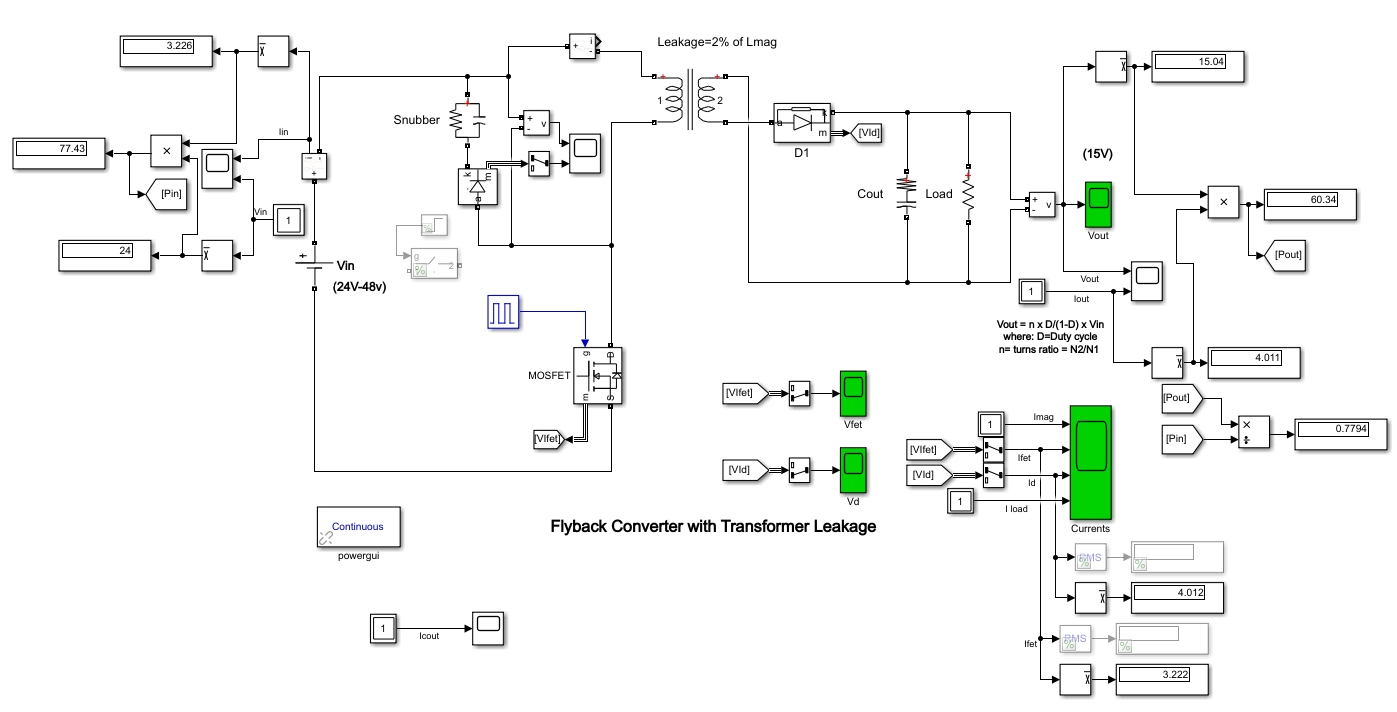
\includegraphics[width=1\textwidth]{figures/24.PNG}
\caption{Efficiency Measurement for 24 V Input Voltage}
\label{fig:eff_24}
\end{center}
\end{figure}

As seen from Figure \ref{fig:eff_24} , efficiency of the flyback converter is 0.779. It is close to the analytical calculations but lower than analytical calculations. At analytical calculations, RMS current and voltage values were calculated by using some approximations. That is why the simulation RMS current and voltage values are different from analytical calculations. So, the efficiency of the system is also measured different because of these differences.There should be additional 5.75 Watt core loss. After core loss is added, efficiency of simulation is given below;

\begin{align}
    \eta = \frac{P_{out}}{P{in}+P_{core}} = \frac{60.34}{77.43+5.75} = \frac{60.34}{83.18} = 0.725
\end{align}
Efficiency of the system is 0.725 when the input voltage is 24.

\subsubsection{Efficiency Analysis from Simulations $v_{in}$ = 36 V}

\begin{figure}[H]
\begin{center}
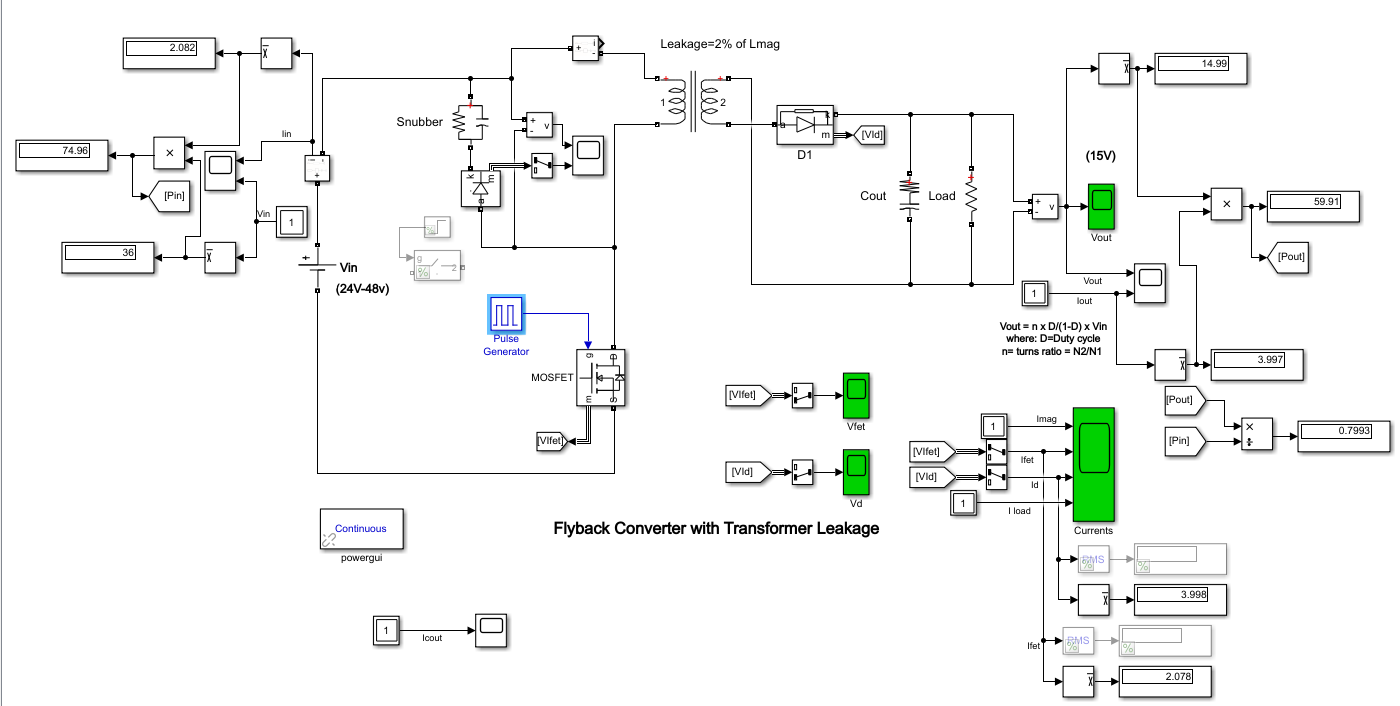
\includegraphics[width=1\textwidth]{figures/36.PNG}
\caption{Efficiency Measurement for 36 V Input Voltage}
\label{fig:eff_36}
\end{center}
\end{figure}

As seen from Figure \ref{fig:eff_36} , efficiency of the flyback converter is 0.799. Which is again so close to the analytical calculations but some differences are observed because of approximations by calculating RMS values.There should be additional 5.75 Watt core loss. After core loss is added, efficiency of simulation is given below;

\begin{align}
    \eta = \frac{P_{out}}{P{in}+P_{core}} = \frac{59.91}{74.96+5.75} = \frac{59.91}{80.71} = 0.742
\end{align}
Efficiency of the system is 0.742 when the input voltage is 36 V.

\subsubsection{Efficiency Analysis from Simulations $v_{in}$ = 48 V}

\begin{figure}[H]
\begin{center}
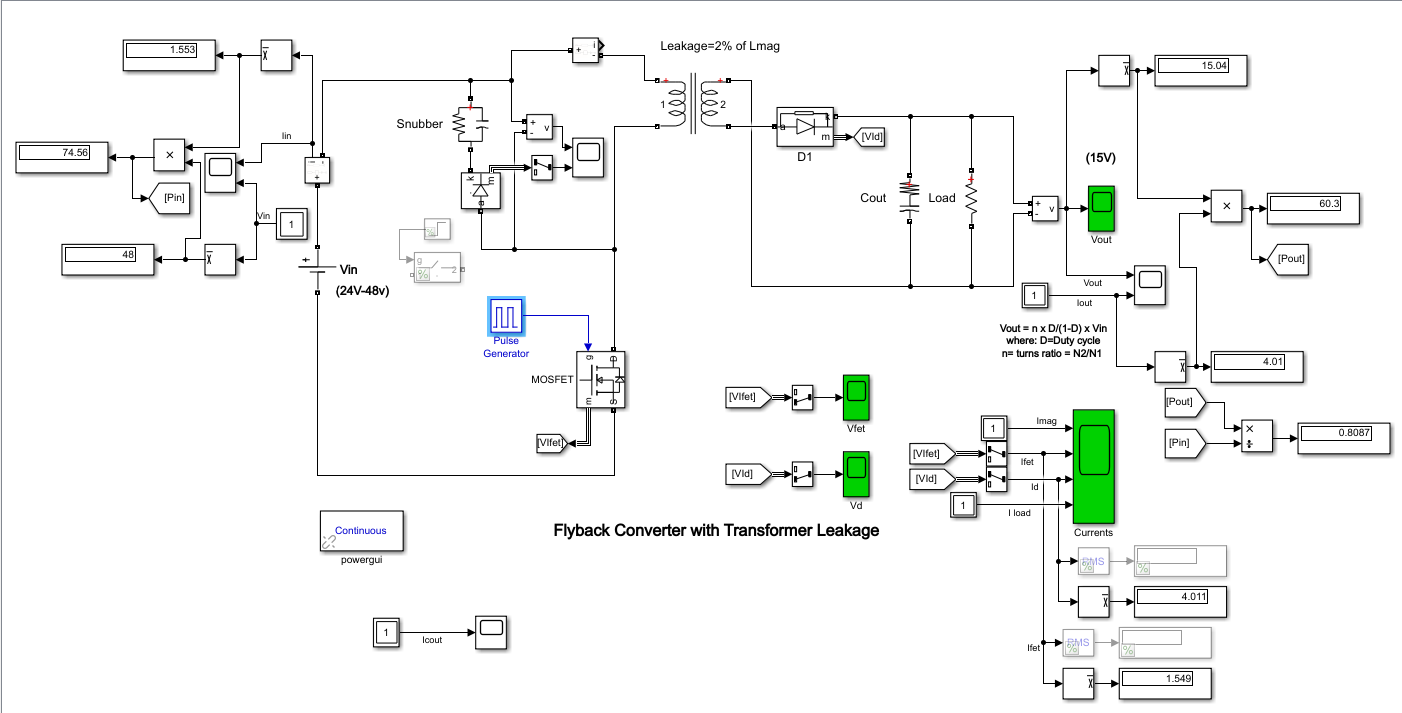
\includegraphics[width=1\textwidth]{figures/48.PNG}
\caption{Efficiency Measurement for 48 V Input Voltage}
\label{fig:eff_48}
\end{center}
\end{figure}

As seen from Figure \ref{fig:eff_48} , efficiency of the flyback converter is 0.808. There should be additional 5.75 Watt core loss. After core loss is added, efficiency of simulation is given below;

\begin{align}
    \eta = \frac{P_{out}}{P{in}+P_{core}} = \frac{60.3}{74.56+5.75} = \frac{60.3}{80.31} = 0.751
\end{align}
Efficiency of the system is 0.751 when the input voltage is 48 V.
As seen from all measurements, efficiency of system is good enough. Most of the losses are caused by MOSFET and diode inertial resistance. These losses can be reduced by using different MOSFET and diodes but chosen components are good enough and economical.


General efficiency analyse comparison is given below;

\begin{table}[H]
\centering
\caption{Efficiency Comparison Table for Analytical Calculations and Simulation Results}
\begin{tabular}{|l|l|l|l|l|}
\hline
Input Voltage & Analytical Efficiency & \begin{tabular}[c]{@{}l@{}}Simulation Efficiency \\ with Core Loss\end{tabular} & \begin{tabular}[c]{@{}l@{}}Analytical Efficiency\\  without Core Lose\end{tabular} & Simulation Efficiency \\ \hline
24 V          & \%74.3                & \%72.5                                                                          & \%79.2                                                                             & \%77.9                \\ \hline
36 V          & \%78.3                & \%74.2                                                                          & \%81                                                                               & \%79.9                \\ \hline
48 V          & \%79.5                & \%76                                                                            & \%83                                                                               & \%81                  \\ \hline
\end{tabular}
\end{table}

\newpage